\documentclass{article}
\usepackage{NotesTeX}
\newgeometry{left=10mm,right=60mm,top=1.5cm,bottom=1.75cm, marginparwidth=5cm, marginparsep=5.25mm}
\usepackage{cleveref}

\usepackage{amsmath}
\usepackage{amsthm}
\usepackage{booktabs}
%\usepackage[lite, subscriptcorrection]{mtpro2}
\usepackage[amsthm, subscriptcorrection]{newtxmath}
\DeclareMathSizes{9 }{9}{6}{4}

%for better bold symbols
\usepackage{bm}
\fancypagestyle{fancynotes}{%
\fancyhf{} % clear existing header/footer entries
\renewcommand{\headrulewidth}{0pt}
\fancyfoot[L]{\thepage}
}%

%load fontspec later, otherwise newtxmath has issues with bold.
\usepackage{fontspec}

%main font
%\setmainfont{Fanwood}[
%  BoldFont={EB Garamond SemiBold},
%  Numbers=Lining,
%  Renderer=Basic
%]
\setmainfont{Baskerville}[
    BoldFont={BaskervilleSemibold}
]
%sans font, for section headings.
\setsansfont{Jost Light}[
  BoldFont={Jost Light},
]
%mono font
\setmonofont{JetBrainsMono}[
  Extension      = .ttf,
  UprightFont    = JetBrainsMonoNerdFont-ExtraLight.ttf,
  ItalicFont     = JetBrainsMonoNerdFont-Italic.ttf,
  BoldFont       = JetBrainsMonoNerdFont-Bold.ttf,
]
%for some reason too large
\newfontfamily\JBMmdfamily{JetBrainsMono}[
  Extension      = .ttf,
  UprightFont    = JetBrainsMonoNerdFont-ExtraLight.ttf,
  ItalicFont     = JetBrainsMonoNerdFont-Italic.ttf,
  BoldFont       = JetBrainsMonoNerdFont-Bold.ttf,
]

%importing integral, sum, and partial symbol from mtpro2
\DeclareFontFamily{U}{mtt}{}
\DeclareFontShape{U}{mtt}{m}{up}{<->mt2exa}{}
\DeclareFontShape{U}{mtt}{m}{it}{<-7> mt2mif <7-9> mt2mis <9-> mt2mit}{}

\DeclareSymbolFont{splgreek}{U}{mtt}{m}{up}
\DeclareSymbolFont{letters}{U}{mtt}{m}{it}

\SetSymbolFont{splgreek}{normal}{U}{mtt}{m}{up}
\SetSymbolFont{letters}{normal}{U}{mtt}{m}{it}

\DeclareMathSymbol{\splsum}{\mathop}{splgreek}{"50}
\let\sum\splsum
\DeclareMathSymbol{\intop}{\mathop}{splgreek}{"52}
\DeclareMathSymbol{\partial}{\mathord}{letters}{64}

%redefinitions because they were acting weird
\renewcommand{\Large}{\fontsize{16}{20}\selectfont}
\renewcommand{\large}{\fontsize{12}{20}\selectfont}
\renewcommand{\LARGE}{\fontsize{22}{40}\selectfont}
\renewcommand{\huge}{\fontsize{30}{60}\selectfont}
\renewcommand{\Huge}{\fontsize{40}{60}\selectfont}
\newcommand{\chapnamefontsize}{\fontsize{36}{44}\selectfont}
\newfontfamily\titlefontish{EB Garamond}



\usepackage[usenames,dvipsnames]{xcolor}
% Other packages which might use the url package.

\hypersetup{
colorlinks=true,
linkcolor=Emerald!50!black,
citecolor=Emerald!50!black,
urlcolor=Emerald!50!black,
}
\bibliographystyle{unsrtnat}
\raggedbottom

\makeatletter
\renewenvironment{thebibliography}[1]
     {\part*{\bibname}% <-- this line was changed from \chapter* to \section*
      \@mkboth{\MakeUppercase\bibname}{\MakeUppercase\bibname}%
      \list{\@biblabel{\@arabic\c@enumiv}}%
           {\settowidth\labelwidth{\@biblabel{#1}}%
            \leftmargin\labelwidth
            \advance\leftmargin\labelsep
            \@openbib@code
            \usecounter{enumiv}%
            \let\p@enumiv\@empty
            \renewcommand\theenumiv{\@arabic\c@enumiv}}%
      \sloppy
      \clubpenalty4000
      \@clubpenalty \clubpenalty
      \widowpenalty4000%
      \sfcode`\.\@m}
     {\def\@noitemerr
       {\@latex@warning{Empty `thebibliography' environment}}%
      \endlist}
\makeatother
\renewcommand{\bibname}{References}

\usepackage{graphicx} % Required for inserting images
\usepackage{parskip}
\usepackage{float} 
\setlength{\parskip}{7pt} % 1ex plus 0.5ex minus 0.2ex}
\setlength{\parindent}{0pt}

\title{2025 Beamline For Schools Experimental Proposal 
{\Large\titlefontish Characterization of and Shielding against Single Event Effects (SEEs) in EEPROMs}   
\vspace{-1em}
}
\author{\large Physics Olympiad Co-operation \\

{\normalfont\large
Adyansh Mishra,  
Akshat Srivastava,
Alexander Fernandez,  
Aryan Prakash,  
Kishore Nanda,
Mia Li,
Ryan Tang,  
Suryachethanreddy Chennamireddy.  
}
}

\date{March 2025}

\begin{document}

\setcounter{section}{1}


\maketitle

\pagestyle{fancynotes}

%\part*{Abstract}
%Single Event Effects are responsible on various electronic failures in %space, and in large colliders like the LHC, where the electronics are %often exposed to heavy ions. We look at various materials to prevent %damage on electronics due to SEEs because of ions of around $\sim$300 MeV %energy. 
\vspace*{-5.5em}
\part{Introduction}

Electronics in space are continuously exposed to cosmic rays—high-energy particles
traveling through space at nearly the speed of light.\sidenote[][7em]{\cite{Scarsi1960Mar} Scarsi, L. (1960). Cosmic radiation. \textit{American Journal of Physics, 28}(3), 213-220. {\footnotesize\url{https://doi.org/10.1119/1.1935104}}} 

The energy spectrum of cosmic rays peaks at approximately 300 MeV.\sidenote[][12em]{\raggedright \cite{Scarsi1960Mar} Scarsi, L. Cosmic radiation.} Of particular concern are the induced \textit{Single Event Effects} (SEEs) at this energy.
SEEs arise when a high-energy particle, either through direct or indirect ionization, produces a charge track within a semiconductor. SEEs can lead to temporary malfunctions or even permanent device failure,\sidenote[][10.9em]{\cite{deAguiar2024Aug} Aguiar, Y.Q.d., Wrobel, F., Autran, JL., García Alía, R. (2025). Introduction to Single-Event Effects. In: \emph{Single-Event Effects, from Space to Accelerator Environments}. Springer, Cham.} depending on the particle's energy.

To analyze a device's vulnerability to such effects, we define the key metric of interest: the \textit{cross section}, $\sigma(E)$.
\begin{equation}
    \sigma (E) = \frac{N_{\text{events}}}{\Phi}, \tag{1}
    \label{eq: sat-cross-section}
\end{equation}

\textit{Equation 1:} Definition of the SEE cross section, where $N_{\text{events}}$ is the number of observed SEE's and $\Phi$ is the fluence---the number of incident
particles per unit area

Typically, the cross section as a function of energy follows a \textit{Weibull distribution}:
\begin{equation}
    \sigma(E) = \sigma_{\text{sat}} \left\{1 - \exp\left(\left(\frac{E - {T\!r}}{W}\right)^S\right)\right\}, \tag{2}
\end{equation}
\textit{Equation 2:} Weibull Distribution of SEE cross section. $\sigma_{\text{sat}}$ is the \textit{saturated cross section} (the asymptotic maximum value at high energies), $T\!r$ is the threshold energy, $W$ is the width parameter, and $S$ is the shape factor.\sidenote{\raggedright \cite{nasa} Edmonds, L. D., Barnes, C. E., Scheick, L. Z. (2000). {An Introduction to Space Radiation Effects on Microelectronics}. \textit{Jet Propulsion Laboratory, California Institute of Technology}. {\footnotesize\url{https://parts.jpl.nasa.gov/pdf/JPL00-62.pdf}}}

Accurately determining $\sigma_{\text{sat}}$ allows us to estimate the cross section at other energy levels.
\begin{figure}[H]
    \centering
    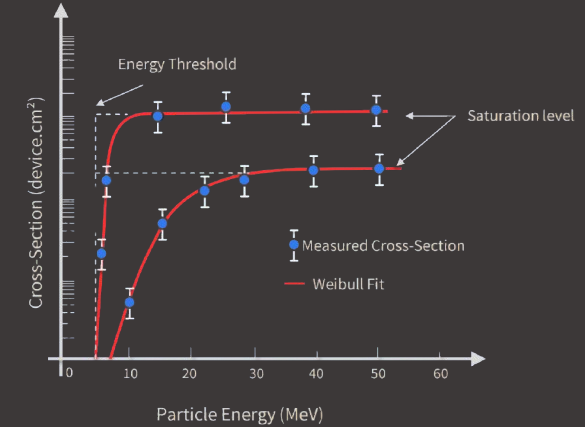
\includegraphics[width=0.5\linewidth]{./graph.png}
    \caption{The cross section $\sigma$ plotted against the particle energy.}
    \label{fig:cross-section}
\end{figure}
We will investigate how various shielding materials can mitigate SEEs. We aim to focus on materials that are inexpensive and easily accessible, enabling cost-effective protection for both spaceborne electronics and accelerator systems such as those at the LHC.

\newpage


\newpage
\vspace*{-5.5em}
\part{Materials}

For shielding, we aim to use a combination of high- and low-density materials to mitigate the effects of both primary and secondary cosmic rays. High-density materials are effective at attenuating primary radiation, while low-density materials help reduce the impact of secondary particles generated by nuclear interactions within the shielding \sidenote[][4em]{\cite{usdept} Navarrete, E. A., Kouzes, R. T., Ankney, A. S., Orrell, J. L., Berguson, T. J., \& Troy, M. D. (2011). Cosmic ray interactions in shielding materials. {\footnotesize\url{https://doi.org/10.2172/1025678}}}. The materials selected for testing include:

\begin{itemize}
    \item \textbf{Concrete}: Due to its density and the possibility of incorporating high-atomic-number aggregates (e.g., barites, magnetites, and hematites), concrete serves as an effective and adaptable shielding material. Its durability and low cost make it ideal for large-scale applications. 

    \item \textbf{Iron}: A dense metal well-suited for shielding against primary cosmic rays. It is lighter than some traditional shielding materials and generates minimal secondary radiation\sidenote[][4.7em]{\cite{usdept} Navarrete, et al. Cosmic ray interactions in shielding materials.}.

    \item \textbf{Aluminum}: Another high-density material, commonly used in spacecraft for radiation shielding. Its widespread use makes it a useful benchmark for comparison with our other candidate materials.

    \item \textbf{Plastic (Polyethylene)}: As a hydrogen-rich, low-density material, polyethylene effectively reduces secondary radiation. It has been successfully deployed as radiation shielding on the International Space Station\sidenote[][0em]{\cite{Durante2014Apr} Durante, M. (2014). Space radiation protection: Destination Mars. \textit{Life Sciences in Space Research, 1}, 2–9. {\footnotesize\url{https://doi.org/10.1016/j.lssr.2014.01.002}}}. It is also affordable and readily available.
\end{itemize}

Additionally, we will be using aerogel with other materials to act as a thermal insulator to protect electronics from heat, forming a mutli-layered shielding setup.

\begin{figure}[H]
    \centering
    \includegraphics[width=0.6\linewidth]{./render4k.png}
    \caption{Multi layered shielding setup, using aerogel, concrete, and a high density metal.}
\end{figure}

\newpage
\vspace*{-5.5em}

\part{Electronics}
For the electronics selected for irradiation, we chose memory chips due to their critical role in nearly 
all digital electronic systems. Specifically, we focused on electrically erasable programmable read-only memory (EEPROM) chips.
EEPROMs are a type of nonvolatile memory that provide greater endurance in terms of read/write cycles and data retention compared to flash memory. 
These reliability characteristics are especially important for space applications, where EEPROMs have been employed in missions such as India's Chandrayaan lunar program. 

EEPROMs operate using floating-gate transistors, which means radiation-induced effects like SEEs are typically localized—causing failures on a per-bit basis rather than device-wide errors.

To ensure compatibility with the beam's constraints, we selected the M95640-WDW6TP EEPROM, manufactured by STMicroelectronics. This device comes in a compact TSSOP-8 package, allowing us to place multiple ICs within the 2 cm diameter of the beam's focal region.
This enables efficient testing through simultaneous irradiation trials.

\vspace{-3em}

\part{Experimental Plan}
To quantify the damage done to the memory chips, we designed a PCB that enables us to write/read data from the M95640. 
Errors in the EEPROM can be detected by writing a known data sequence to memory, irradiating the chip, and then 
reading the data back to identify any discrepancies. Finally, we will attempt to reprogram and read from the EEPROM without
irradiation to check for the presence of any “stuck bits”---memory values that are permanently stuck and can no longer be 
changed. A greater number of stuck bits indicates a higher level of damage to the chip.

\begin{figure}[H]
    \centering
    \includegraphics[width=0.6\linewidth]{./PCB.png}
    \caption{Interface PCB for M95640-WDW6TP}
    \label{fig:enter-label}
\end{figure}


\section*{EEPROM Initialization and Irradiation Scheme}

We will initialize all memory addresses of the four EEPROM chips with an alternating sequence of $1$s and $0$s. The chips will then be 
irradiated at CERN's T9 beamline using the positively charged beam, 
selecting particles with momenta between $0.6$ GeV/$\mathrm{c}$ and $0.9$ GeV/$\mathrm{c}$. 

This momentum range ensures the beam includes protons with energies between approximately 
$200-300$ MeV, and pions, kaons with higher energy, allowing us to measure the saturated cross-section. 
It also replicates the typical energy spectrum of cosmic rays.\sidenote{\cite{Scarsi1960Mar} Scarsi, L. Cosmic Radiation.} 

At this beam momentum, the total flux is sufficient to induce observable effects on the chips. 

The irradiation will last for $10$ minutes under continuous exposure to the T9 beam. 
After irradiation, we will read out the data from all memory addresses to determine the number of bits that flipped from their original values.

Finally, we will invert every bit in memory (i.e., flip all $1$s to $0$s and all $0$s to $1$s), and then read the memory
again to identify bits that failed to flip correctly.

\section*{Evaluating Candidates for Shielding Materials}

We aim to evaluate the effectiveness of various low-cost shielding materials in protecting against Single Event Effects (SEEs).
\begin{table}[h]
\caption{Overview of experimental parameters for the shielding materials being tested}
\vspace*{2.5mm}
\label{table:experimental}
\begin{tabular}{@{}lllll@{}}
\toprule
\multicolumn{1}{c}{\textbf{Material Tested}} & \multicolumn{1}{c}{\textbf{\begin{tabular}[c]{@{}c@{}}Thickness\\ (cm)\end{tabular}}} & \multicolumn{1}{c}{\textbf{Number of Trials}} & \multicolumn{1}{c}{\textbf{\begin{tabular}[c]{@{}c@{}}Beam Momentum\\ (GeV/c)\end{tabular}}} & \multicolumn{1}{c}{\textbf{\begin{tabular}[c]{@{}c@{}}Irradiation Time\\ (min)\end{tabular}}} \\ \midrule
\multicolumn{1}{l}{No shielding (Control)} & \multicolumn{1}{l}{N/A}                                                              & \multicolumn{1}{l}{10}                       & \multicolumn{1}{l}{0.6 - 0.9}                                                               & \multicolumn{1}{l}{10}                                                                       \\ 
\multicolumn{1}{l}{Concrete}               & \multicolumn{1}{l}{10}                                                               & \multicolumn{1}{l}{10}                       & \multicolumn{1}{l}{0.6 - 0.9}                                                               & \multicolumn{1}{l}{10}                                                                       \\ 
\multicolumn{1}{l}{Iron}                   & \multicolumn{1}{l}{10}                                                               & \multicolumn{1}{l}{10}                       & \multicolumn{1}{l}{0.6 - 0.9}                                                               & \multicolumn{1}{l}{10}                                                                       \\ 
\multicolumn{1}{l}{Aluminum}               & \multicolumn{1}{l}{10}                                                               & \multicolumn{1}{l}{10}                       & \multicolumn{1}{l}{0.6 - 0.9}                                                               & \multicolumn{1}{l}{10}                                                                       \\ 
\multicolumn{1}{l}{Polyethylene}           & \multicolumn{1}{l}{10}                                                               & \multicolumn{1}{l}{10}                       & \multicolumn{1}{l}{0.6 - 0.9}                                                               & \multicolumn{1}{l}{10}                                                                       \\ \bottomrule
\end{tabular}
\end{table}

\section*{Data Analysis}

For each irradiation run, we will record the number of SEEs, specifically tracking Single Event Upsets (SEUs) and Single Event Latch-ups (SELs). 
Additionally, we will calculate the beam fluence, enabling us to determine the saturated SEE cross section of the EEPROM given by \Cref{eq: sat-cross-section}

To assess whether a given shielding material significantly reduces the SEE cross section compared to the unshielded control, we will use a two-sample $t$-test with a significance level of $p = 0.01$.
\begin{equation}
t = \frac{\bar{\sigma}_{\mathrm{o}} - \bar{\sigma}_{\mathrm{e}}}{\sqrt{{s_{\mathrm{o}}^2}/{n_{\mathrm{o}} + {s_{\mathrm{e}}^2}/{n_{\mathrm{e}}}}}} \tag{3}
\end{equation}
\noindent
\textit{Equation 3:} Two-sample $t$-statistic comparing the mean SEE cross sections $\bar{\sigma}_{\mathrm{o}}$ (control) and $\bar{\sigma}_{\mathrm{e}}$ (experiment), with sample variances $s_{\mathrm{o}}^2$ and $s_{\mathrm{e}}^2$ and sample sizes $n_{\mathrm{o}}$ and $n_{\mathrm{e}}$ respectively.

From this, we will determine which of the shielding materials tested are statistically effective in reducing the SEE cross section in EEPROM devices.

\newpage
\vspace*{-5.5em}

\part{Motivation}

\subsection*{Why We Want To Go}

We are a group of eight students from India and USA, involved in the shared community of olympiad physics. 
This journey has introduced us to new fields outside of the olympiad physics.

Getting to work hands on and see our experiment come to life would act as a catalyst for both ourselves and others
to pursue particle physics and related fields in the future, helping us promote physics research in our countries.

Our proposal would allow us to experiment various shielding materials, some of which are not regularly used for shielding
from SEEs. Seeing it come to fruitition would allow us to contribute into 
ensuring electronic safety in places like LHC and space satellities.

\subsection*{What We Hope To Gain}

We hope to go to CERN to work on our experiment, beyond the the theoretical work we've been engaged in for the 
past months, which would introduce to real word experience in experimental physics and the scientific method in general.  

This would also enable us to interact with those working in the field and peers worldwide, and give us a peek into what's ahead.

\vspace{-3em}
\part*{Acknowledgments}

We would like to thank our coach Yash Mehta, MS in Physics at IISc Bangalore, for his guidance and funding the writing of the proposal.
We would additionally like to thank Dr. Gunn Khatri, Applied Physicist at CERN, for his advice and guidance.

\newpage
\vspace*{-5.5em}
\bibliography{refereces}

\end{document}
